% 1274 words

\subsection{Key Questions}
what was the scope and how was it defined
what filters were used
what were the walking and cycling speeds used
what were the travel times calculated
what was the directness of travel on different networks
what is the distribution of travel times in the different networks
what lsoas changed the most and least across networks
how did removing road types affect the number of lsoa centers connected?
how long did the calculations take?
Did removing directionality from the networks have a significant effect?
Did removing directionality mediate the effect of removing primary and trunk streets?



\subsection{Defining Scope}


Goal is to capture the largest computationally feasible network with a simple set of rules. 

The first rule was to restrict the network to ``inner london''. This has the advantage of a formal designation by the GLA for each borough, capturing, XXX\% of the population with a population density of XXXXXX compared to XXXXX for london overall, XXXXXX\% of the jobs in the city, and XXXX\% of the journey's to work. Additionally, rates of cycling are higher in inner London than in the periphery. 

Second, the area of interest was restricted to north of the river Thames. This captures XXX\% of the population, with a density of XXXXXXX, XXX\% of London's jobs, and XXX\% of the journey's to work. Further, it has the advantage of excluding the need to cross the river, where journey's are focused on a few number of bridges, with a significant effect on the shortest paths, reducing the effect of other changes on the network. 

\begin{table}[]
\centering
\begin{tabular}{lcccl}
 Mode Share Within Scope & All Modes & Bicycle & \% by bicycle &  \\
 \hline
 Origin in scope &  981,354 & 46,832 & 4.8\% &  \\
 Destination in scope & 1,454,606 & 48,461 & 3.3\% &  \\
 Both in scope & 479,882 & 24,843 & 5.2\% & \\
 All journeys & 5,852,298 & 140,180 & 2.4\% \\ 
\end{tabular}
\caption{commuter data}
\label{table:commute_data}
\end{table}

text

\subsection{Defining Networks}

\subsubsection{Level 1}

\subsubsection{Level 2}

\subsubsection{Undirected}

\subsubsection{Levels 3, 4, and 5}


Level\_5

no interaction with cars
because this was a negative filter many nodes were excluded needlessly. 
check this, why isn't the regents bike path fully included?


\subsubsection{Misc}

Five network definitions were considered. The exact filters used to select this data are available in APPENDIX XXXX 

The first network is the set of edges where a cyclist can expect to travel without interacting with motorized traffic at all. This is separated cycle routes, tow paths, and other segregated ways. 

The second builds on the first by adding ways tagged as living streets and residential streets.

The third adds all public streets where cycling is not forbidden. 

The fourth network is an undirected version of the third network. This is used to consider the effect of one way restrictions on travel times. 

The fifth network is made up of the cycleways designated by TfL on Open Street Map. This is an interesting case because a significant part of this network is made of routes without cycle infrastructure. The network is considered in the sense that, if this was to become a high quality, low stress network, how well would it serve journeys in London? 


Building networks using Overpass API queries proved to be a tremendous challenge. There are two possible approaches to building an Overpass query filter, positive and negative filters. OSMnx relies on negative filters, including everthing but what is specifically excluded. This was the type of filter used for the 5 levels of networks studied, with more conditions added to take out additional highway types. The trouble that arises with a negative filter though is that an edge that is tagged, highway = primary, and tagged separately with a cycle related tag will be excluded. This was a problem for instance where cycle infrastructure was tagged, not as a separate edge, but as metadata using for instance "cycleway:left=lane" key value pair. the negative filter removes the edge because it has the "highway=primary" tag and a method for including based on the cycle tag was not found. Likewise, the "bicycle" key could have several values including no, designated, and permissive

Further, OSMnx retrieves ways with a highway tag as in way[highway=cycleway]

This ruled out using the filter relation[route=bicycle]  which would collected all nodes and ways included in any relation tagged with route-bicycle. 

Thus the networks built using a  full combination of conditions were not possible. 

good example of the difficulty of building a good network representation is castle baynard st. It connects the central london part of cycle superhighway 3 with the east london section that continues out to limehouse. this is a tunnel that serves as a bike path and as a driveway of sorts to an underground car park. 

insert picture of castle baynard street. A network built from the relation[route=bicycle] set of ways and nodes would include this but the negative filters do not. 



Each network is created using a filter that excludes Open Street Map features tagged with certain values. All features tagged with ``bicycle=no'' or ``service=private'' were excluded. Additionally, where the edge's ``highway'' tag was ``footway, steps, corridor, elevator, escalator, motor, proposed, construction, abandoned, platform, or raceway the feature was also excluded. 

The most aggressive bike filter used only these conditions.


\subsubsection{London's OSM data}

\subsubsection{Filters used}

\begin{figure}
  \centering
  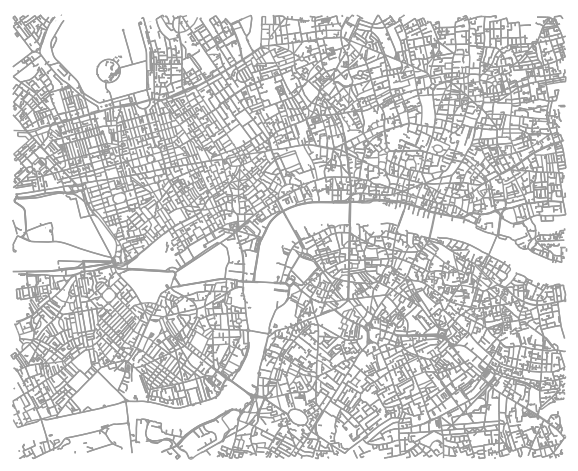
\includegraphics[width=0.5\linewidth]{bbox_bike_1_filter_cropped}
  \caption{1: most confident cyclists}
  \label{fig:sub1}
\end{figure}

\begin{figure}
  \centering
  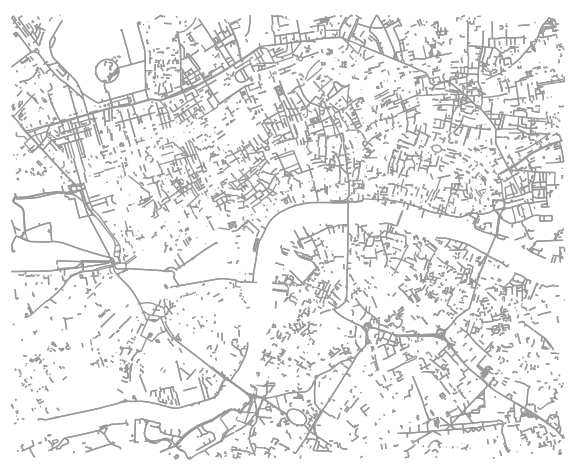
\includegraphics[width=0.5\linewidth]{bbox_bike_5_filter_cropped}
  \caption{5: no interaction with cars }
  \label{fig:sub2}
\end{figure}



\begin{figure}
  \centering
  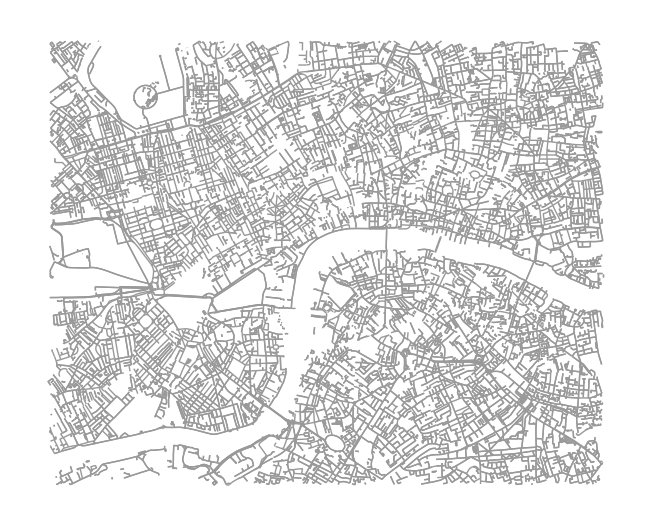
\includegraphics[width=0.5\linewidth]{bbox_bike_2_filter_cropped}
  \caption{2: all but primary and trunk streets}
  \label{fig:sub2}
\end{figure}



\begin{figure}
  \centering
  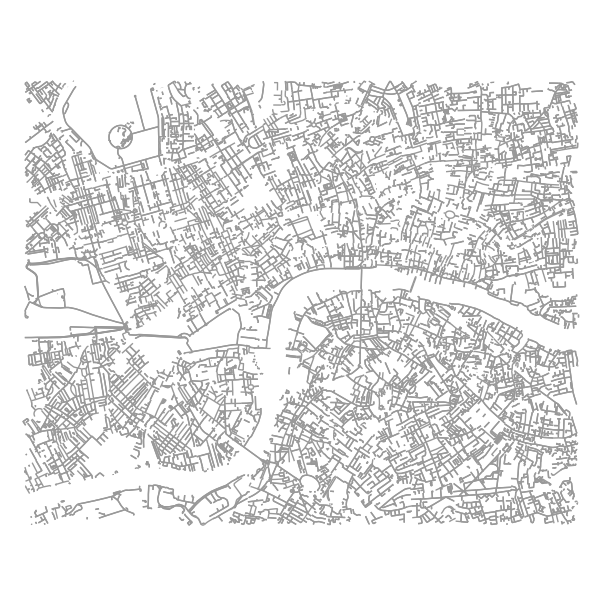
\includegraphics[width=0.5\linewidth]{bbox_bike_4_filter_cropped}
  \caption{4: only residential and living streets}
  \label{fig:sub2}
\end{figure}


\subsubsection{Quant Network}

Quant has 23,377,225 pairs. The subset has 799,236. The subset has 200,041 missing distances. 

To complete the missing distances, the quant travel times were built into a networkx multidigraph. There was an edge for each node pair that represented the walking time between the nodes, calculated as the straightline distance between the nodes divided by the google walking speed 3 mph converted to 4.83 kph and converted to  0.0805 kilometers per minute giving a number of minutes walking time between the nodes that was in the same units as the number of minutes public transit time between the nodes. 

Then for each pair of nodes missing a transit time, the shortest path on the graph was calculated. Thus each travel time can be a combination of walking and riding public transit between nodes. 


\subsection{Network Characteristics}

chart of largest connected component of network as edge types are included. 

\begin{figure}
\centering
\caption{largest component of network type}
\label{fig:connected_component}
\end{figure}

no cars,
+ living streets
+ residential streets
+ tertiary 
+ secondary
+primary

\begin{table}
\centering
\caption{table of network statistics}
\label{table:network_stats}
\end{table}

\subsection{Defining Origins and Destinations}

Node 5816785884, closest to the centroid of LSOA XXXXXX is found at the entrance to a garage at the end of a one way street. Thus every other node in the network is inaccessible on the directed versions of the network. The edge leading to this node is tagged ``service'' so perhaps service streets should have been excluded as they are frequently dead ends. 

\begin{figure}
\centering
\caption{histogram of distances between centroid and nearest common node. }
\label{fig:centroid_node_dist_hist}
\end{figure}

Because urban density increases as one approached the center of a city, there may be a slight bias towards node distances being lower than centroid distances. This is because there is a higher probability that the closest node will be on the central side of the centroid than the outside. 



\begin{figure}
\centering
\caption{distribution of differences between Quant distances and Cycle Origins and Destinations}
\label{fig:diff_dist}
\end{figure}

\subsection{Travel Times}

Travel times were converted from distances using a walking speed of 3 mph and a cycling speed of 8 mph based on data taken from google maps estimates for journeys as seen in that table. 

\begin{table}
\centering
\caption{Google Maps travel speeds}
\label{table:travel_speeds}
\end{table}

As seen table XXXXX travel times for bike network 2, without trunk or primary highways, are substantially longer than travel times for bike network 1. This indicates that the effect of removing these edges is not just to disconnect the network but also requires a network user to take a less direct route, straying further from the straight line between origin and destination. 

The difference between directed and undirected distances is also notable. 

the standard deviation 

the min is unchanged, while the max 

Travel times by bicycle for aggressive cyclists are XXXXX compared to the QUANT travel times by public transport. 

\subsubsection{test for differences}

There's got to be a significant difference between the distances for the different networks right?


\begin{table}
\centering
\caption{google speed estimates}
\label{table:google_speeds}
\end{table}


\begin{table}
\centering
\caption{travel time statistics}
\label{table:travel_time_stats}
\end{table}

\subsection{Changes in Routing}


\subsubsection{compare route across directedness}
\begin{figure}
\centering
\caption{example of routing on directed network 1}
\label{fig:routing_1}
\end{figure}

\begin{figure}
\centering
\caption{example of routing on undirected network 1}
\label{fig:routing_1}
\end{figure}

\subsubsection{compare route across level 1 and 2}

Seen in figure XXXX  compare longest path for directed network 2 to the path between those nodes in directed network 1. 

Compare longest path for directed network 1 to undirected network 1. 

compare o/d pair with largest increase in distance between directed 1 and directed 2 to the distance in undirected 2. 

Is allowing travel in any direction on side roads a good replacement for primary and trunk routes?


\begin{figure}
\centering
\caption{example of routing on directed network 1}
\label{fig:routing_1}
\end{figure}

\begin{figure}
\centering
\caption{example of routing on directed network 2}
\label{fig:routing_1}
\end{figure}

\subsubsection{compare across level 2 directedness}

\begin{figure}
\centering
\caption{example of routing on directed network 2}
\label{fig:routing_1}
\end{figure}

\begin{figure}
\centering
\caption{example of routing on undirected network 2}
\label{fig:routing_1}
\end{figure}


\subsection{Accessibility}

in qgis, color lsoa's by travel time to central lsoa. 

in QGIS color lsoa's by travel time from lsoa with highest average distance. 

in QGIS color lsoa's by  average directness, distance divided by straightline distance. 

Plot a few paths in osmnx to look at low directness. 


\begin{figure}
\centering
\caption{lsoas colored by directness of routes to other lsoas}
\label{fig:lsoa_directness}
\end{figure}



\subsection{Notes about computation}

runtimes for the distances between nodes were long. computations were done on an intel i74700HQ processor with the database contained on the internal Solid State Drive. 

Runtimes increased with the number of connected origin destination pairs, since unconnected pairs  did not require the calculation of a shortest path. Thus bike 1 travel times took longer than bike level 2. Additionally, the undirected network calculations took substantially longer than the directed networks because there were sugnificantly more route possibilities with more edges available at each node. 

Table XXXX contains calculation times by network type. 

% table for computation times across algorithm types

% table for computation times across network types
%\begin{table}[]
%\centering
%\begin{tabular}{lllll}
%network  & 1 & 1 undirected & 2  & 2 undirected   \\
%time     & 24:00   & 72:00??  & 9:03  & 36:00        \\        
%\end{tabular}
%\caption{Computation Times}
%\label{table:1}
%\end{table}

\begin{table}[]
\centering
\begin{tabular}{@{}l|llll@{}}
network     & 1           & 1 undirected & 2    & 2 undirected \\ \hline
time(hours) & $\sim$24:00 & $\sim$72:00  & 9:03 & $\sim$36:00 
\end{tabular}
\caption{Calculation times for routes}
\label{table:net_calc_times}
\end{table}

\begin{table}
\centering
\caption{computation times using different algorithms}
\label{table:comp_times_algo}
\end{table}


text